\documentclass[11pt]{article}
\usepackage{epsfig}
\input shared.texm
\startfile
\begin{pspicture}(-2,-2.3)(4,3.3)
\def\MNODE(#1,#2)#3#4{%
\cnode(#1,#2){0.31}{#3}\rput(#1,#2){#4}}%
\def\PNODE(#1,#2)#3{%
\cnode[fillstyle=solid,fillcolor=black](#1,#2){0.1}{#3}}%
\def\XA{-2.5}\def\XB{-1.5}\def\XC{0}\def\XD{1}
\def\XE{3}\def\XF{4}
\def\XP{\XA}\def\YP{-2.2} %pnode 
\def\XX{0.2} %dist of sunflower legs
\def\YDO{0}
\def\YA{1}
\def\YSA{1.9}
\def\YSB{0.3}
\def\YSC{-1.6}


\def\SF(#1,#2)#3#4{%
\rput[b](#1,#2){\pnode(-\XX,0){R#3#4S}\pnode(\XX,0){R#3#4E}
\rput[b](0,1.0){$R_{#3,#4}$}
\rput[b](0,0){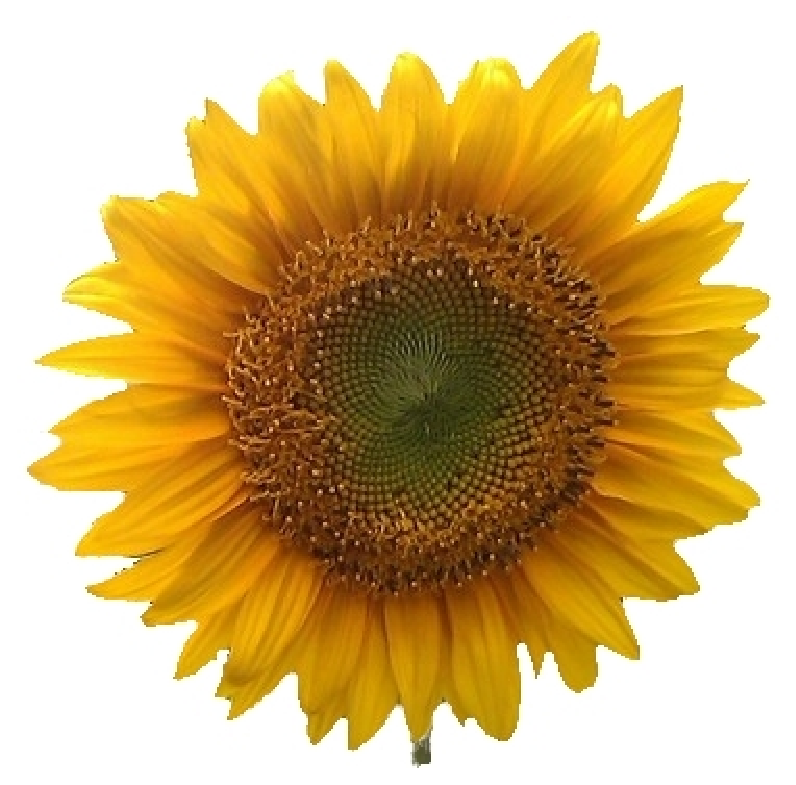
\includegraphics[width=1cm]{sunflower.eps}}
}}

\MNODE(\XA,0){M}{$M$}
\MNODE(\XB,-\YA){IY}{$I_Y$}
\MNODE(\XB,\YA){IX}{$I_X$}
\MNODE(\XB,\YA){IX}{$I_X$}
\PNODE(\XC,0){RS}
\PNODE(\XF,0){RE}
\pnode(\XP,\YP){P}

\SF(\XD,\YSA){1}{X}
\SF(\XD,\YSB){2}{X}
\SF(\XD,\YSC){k}{X}
\SF(\XE,\YSA){1}{Y}
\SF(\XE,\YSB){2}{Y}
\SF(\XE,\YSC){k}{Y}

\rput(\XD,\YDO){\large \dots}
\rput(\XE,\YDO){\large \dots}

\psset{arrows=->,linecolor=darkgray}
\ncline[arrows=<->]{M}{IY}
\ncline[arrows=<->]{M}{IX}
\ncline[arrows=<->]{IX}{IY}
\ncline{IX}{RS}
\ncline{IY}{RS}
\ncline{M}{RS}
\nccircle[angle=90,nodesep=-1pt]{M}{0.3}
\nccircle[angle=0,nodesep=-1pt]{IX}{0.3}
\nccircle[angle=-135,nodesep=-1pt]{IY}{0.3}

\ncarc[arcangle=15]{RS}{R1XS}
\ncline{RS}{R2XS}
\ncarc[arcangle=-15]{RS}{RkXS}
\ncline{R1XE}{R1YS}
\ncline{R2XE}{R2YS}
\ncline{RkXE}{RkYS}
\ncarc[arcangle=15]{R1YE}{RE}
\ncline{R2YE}{RE}
\ncarc[arcangle=-15]{RkYE}{RE}

\ncdiagg[arrows=-,angleA=-90, armA=2, linearc=0.5]{RE}{P}
\ncline{P}{IY}
\ncline{P}{IX}
\ncline{P}{M}

\end{pspicture}
\endfile
